\chapter{Discussion of the overall thesis and outlooks}
\label{ch:discussion}
%Here we really discuss what is the contribution of the thesis in the global scope of glacial outburst flood. In that sens this more an outlook chapter than a pure discussion (point-specific discussions are present at the end of each chapter). We take perspective and implement all the different bits of this thesis in the worls of GLOFs

\section{New insights on the choice of the Nusselt parametrization during supraglacial lake drainage and the problem of the characteristic length}

In Chapter~\ref{ch:chapter_plainemorte} (published as \cite{Ogier&al2021}), our thermodynamic analysis of the supraglacial channel at Lac des Faverges (see Section~\ref{sec:thermodynamics_results} and \ref{sec:thermodynamics_discussion}) shows that the Nusselt numbers obtained using the Dittus-Boelter equation differ from those predicted by previous studies \citep{Lunardini&al1986, Clarke2003, Vincent&al2010}. These studies also employed the Dittus-Boelter equation but with different empirical coefficients. The discrepancies on the coefficient values suggest that these coefficients should be treated as stochastic variables in future modeling, highlighting the lack of consensus on their appropriate values. Our study calls for more in situ field measurements characterizing the heat transfer during supraglacial drainage.

In 2023, a situation similar to the drainage event at Lac des Faverges occurred at Glacier des Bossons (Mont Blanc, France). An ice-margin lake, formed initially in 2015, had grown significantly and posed a potential threat to downstream populations. Consequently, authorities decided to drain the lake during the summer of 2023 through an artificially-dug supraglacial channel. 

Inspired by the monitoring methods described in \cite{Ogier&al2021}, scientists from IGE Grenoble conducted extensive field measurements detailed in \cite{Gagliardini&al2024}. Their objective was to gain deeper insights into the hydraulics and the thermodynamics of such drainage events, particularly focusing on the processes of channel erosion driven by the water flow, which control the lake discharge. The variables continuously recorded were the lake level, the lake temperature, and the water temperature at four locations within the channel. Additionally, discontinuous records of streamflow discharge and channel floor topography were acquired. The total lake emptying (12500$m^3$) took less than a week, resulting in a channel erosion of 6 meters.

The aim of the monitoring network was to feed and validate the supraglacial drainage model developed in \cite{Vincent&al2010}. This model focuses on simulating the erosion (i.e.\ the ice melt rate) at the ice spillway where lake water enter. The erosion process is primarily driven by heat transfer from water to ice (see Equation~\ref{eq:melt-rate} in Chapter~\ref{ch:chapter_plainemorte}), leading to ice melting and the consequent lowering of the ice dam spillway. The model assumes a uniform melt along the channel and a rectangular cross-section with a constant width, which aligns with observations made at Plaine Morte in 2019 (see Figures~\ref{canal_profile} and \ref{fig:picture_channel}). In particular, the model is capable of implementing the various Nusselt parametrizations proposed in \citep{Clarke2003, Vincent&al2010, Ogier&al2021} for calculating heat transfer to the ice walls of the supraglacial channel. 

% stability of the Bossons drainage?

%the width of the channel in Bossons varies, unlike the (relatively) uniform widths observed in \cite{Vincent&al2010,Ogier&al2021}. The channel width is an important parameter in the drainage hydraulics, influencing both the Reynolds number in Equation~\ref{eq:reynolds} and the Nusselt number in Equation~\ref{eq:nusselt} (see Section~\ref{sec:methods} in Chapter~\ref{ch:chapter_plainemorte}). In particular, narrow channels result in higher discharge rates \todo{cite report of GAG for the sake of this section}.

Results of the application of the lake drainage model described above to the field data acquired at Lac des Bossons indicate that the highest uncertainty in the channel floor evolution comes from the choice of the Nusselt parametrization \cite{Gagliardini&al2024}. This choice is important because it directly impacts the calculation of the outflow discharge. These parametrization used in the model are the Dittus-Boelter parametrization with the empirical coefficients of \cite{Clarke2003,Vincent&al2010,Ogier&al2021} (see Table~\ref{table:DBcoefficients} in Chapter~\ref{ch:chapter_plainemorte}) and the Gnielinski parametrization (see Equation~\ref{eq:Gnielinski} in Chapter~\ref{ch:chapter_plainemorte}) with the the friction factor ($f_D$) equal to 0.3 (see Table~\ref{table:friction_factor} in Chapter~\ref{ch:chapter_plainemorte}). In order to find the most adequate Nusselt parametrization for the Lac des Bossons drainage, \cite{Gagliardini&al2024} compared the Nusselt parametrization mentioned above to their field observation, in particular to the observed channel floor elevation and the lake level elevation. 

\begin{figure}[h]
    \centering
    \includegraphics[width=1\textwidth]{chapters/Discussion/Bossons_models.pdf}
    \caption{Results from \cite{Gagliardini&al2024} (with permission). Observed lake level ($z_L$) and channel-floor entrance elevation ($z_b$), and modeled lake level (continuous line) and channel-floor entrance elevation (dashed line) for a) $\lambda\,=\,w$ and b) $\lambda\,=\,D_H$ according to the different Nusselt parametrization. The Gnielinski parametrization is used for $f_D$\,=\,0.3. GNSS means Global Navigation Satellite System. The RMSE (m) for the model fit to the observations is provided in parentheses for each Nusselt parametrization.}
    \label{fig:gag_nusselt}
\end{figure}


Figure~\ref{fig:gag_nusselt}a shows that the best fit between the modeled and the observed channel erosion is achieved by using the Gnielinski parametrization with the mean friction factor ($f_D\,=\,0.3$) measured in \cite{Ogier&al2021} (RMSE = 0.17). Indeed, if considering typical lower fiction factor (e.g. $f_D$\,=\,0.01 to 0.03 in \cite{Ancey&al2019}), the Gnielinski parametrization is then equivalent to the Dittus-Boelter parametrization for the parameter values given in \cite{Clarke2003}, which leads to a underestimation of channel incision (not shown). However, we showed in Chapter~\ref{ch:chapter_plainemorte} that the friction factor varies by a factor of three during the drainage, and it was possible to establish a correlation with other parameters (e.g. such as Reynolds number, Figure~\ref{fig:Re_Nu} in Chapter~\ref{ch:chapter_plainemorte}), preventing any attempt for a empirical parametrization. The variability of $f_D$ was also highlighted by recent field investigation \citep{pohle&&2022}, which showed a range of value from 0.1 to 13 in an englacial R-channel. This suggest that a single friction factor, assumed to be constant in both space and time, cannot adequately parameterize the dissipation of energy in both supraglacial and subglacial channels, which is in agreement with our findings.

In the calculation of the channel erosion, it is necessary to define a characteristic length ($\lambda$) over which the heat transfer is applied (see Equation~\ref{eq:melt-rate}). \cite{Gagliardini&al2024} considered the channel width ($w$) as the characteristic length for the melt rate calculation, which is also the case in \cite{Vincent&al2010}. In \cite{Clarke2003,Ogier&al2021,Sommers&Rajaram2020}, this characteristic length is equal to the hydraulic diameter $D_H$ (as for the calculation of the Reynolds number), and in \cite{Walder&Costa1996} the characteristic length is equal to the wetted perimeter. The debate on the choice of $\lambda$ highlights the need to better understand the influence of this parameter on the drainage model results.

\cite{Gagliardini&al2024} explored an alternative scenario where $\lambda = D_H$ (instead of $\lambda = w$) in Equation~\ref{eq:melt-rate} to determine the melt rate of the channel floor. They found that in this case, the best match with their observations was not achieved with the Gnielinski parametrization (see Fig.~\ref{fig:gag_nusselt}a), but rather with the Dittus-Boelter parametrization using the empirical coefficient obtained in \cite{Ogier&al2021}. In conclusion, the choice of the characteristic length in the heat flux equation cannot be made independently of the choice of the Nusselt parametrization. 


The Nusselt parametrization proposed in \cite{Ogier&al2021} and discussed in \cite{Gagliardini&al2024} has been also assessed in \cite{pohle&&2022}. The authors compared temperature measurements in a englacial R-channel with predictions from various Nusselt parametrizations \citep{Lunardini&al1986, Clarke2003, Vincent&al2010, Sommers&Rajaram2020, Ogier&al2021} and found a good agreement with those proposed by \cite{Ogier&al2021} and \cite{Vincent&al2010} and mediocre with \cite{Lunardini&al1986,Clarke2003,Sommers&Rajaram2020}. Unfortunately, \cite{pohle&&2022} couldn't quantifying their own Nusselt parametrization as in \cite{Ogier&al2021} due to temperature measurement inaccuracies. 

In conclusion, these findings suggest a need for unified modeling frameworks for heat transfer in supraglacial drainage. Given the variability observed in the friction factor and Nusselt number discussed in this thesis, it is prudent to treat these variables as stochastic in modeling frameworks. By this mean, it will be possible to give a range of possible drainage scenario in future supraglacial lake drainage. We encourage independent modelling studies \citep[e.g.][]{Jarosch&Gudmundsson2012,Kingslake&al2015} to use the recent dataset of supraglacial lake drainage \citep[e.g.][]{Vincent&al2010,Ogier&al2021,Gagliardini&al2024} and to conduct sensitivity analysis of the relevant parameters (i.e.\ which control the lake discharge), with a strong focus on the Nusselt number parametrization and the associated characteristic length. 


\section{Bias in reporting water pocket outburst flood: an example of the hypothetical case of Rhonegletscher in 2022}


In the Chapter~\ref{ch:chapter_WPOFs}, we proposed four mechanisms of water pocket formation leading to water pocket outburst floods (WPOFs). One of them (the most common according to our WPOFs inventory) is the formation of a water pocket caused by the development of a subglacial cavity, that can potentially lead to the partial or total collapse of the ice roof above the cavity (see Fig.\ref{fig:IceBlockage}a). 

We monitored such a development of subglacial cavity and its collapse in the summers of 2022/2023 at Rhonegletscher (Switzerland)(see Fig.~\ref{fig:WP_rhone}a), although we don't have evidences for an outburst prior to the detection of the cavity. Our monitoring program, initiated in June 2022, included mass balance measurements, repetitive topography measurements by UAV, GPR surveys (that I conducted), and visual inspections through boreholes. This dataset was presented in conferences \citep{Ogier&al2022,Hosli&al2022,Bauder&al2023} and  will be part of a future publication led by Hösli (in preparation). In this discussion, we are interested on the GPR measurements performed over the cavity on July 28th 2022, which indicated a cavity volume of approximately 5000\,m$^3$ and confirmed that the cavity was empty (i.e., air-filled). Taking this opportunity, I discuss here the potential for the subglacial cavity to cause a WPOF and consider whether such an event would have been detectable further down in the proglacial lake. Indeed, the lake might dampen the hydrological signal, reducing the peak discharge and potentially preventing the detection of a water pocket outburst flood. 

To discuss on a possible WPOF from Rhonegletscher, I modeled the hypothetical instantaneous drainage of the 5000\,m$^3$ subglacial directly into the lake (i.e.\ I don't consider the distance between the cavity and the lake) and compute the lake outflow by applying the principle of mass conservation. First, the lake outflow $Q_{\rm out}$ (m$^3$\,s$^{-1}$) is initialized for a given lake level height $h_{\rm lake}$ above the spillway elevation (the elevation reference). The relationship between $Q_{\rm out}$ and $h_{\rm lake}$ is obtained by a stage-discharge relationship written as $Q = a\,\times\,h_{\rm lake}$, where $a$ is a fitted parameters (the lake walls are assumed vertical for such low value of lake height variation, i.e.\ few tens centimeters at most). The coefficients $a = 0.044$ was obtained from discrete field measurements of lake level (by GPS) and lake outflow (by salt dilution experiments) acquired at the same time during a field course organized in the frame of the "applied glaciology master" at ETHZ in August 2022 (not shown here, see also similar method described in Section~\ref{subsubsection:Hydraulics} in Chapter~\ref{ch:chapter_plainemorte}). In a second step, the lake outflow is computed by implementing the lake input (i.e.\ the lake recharge from icemelt) $Q_{\rm in}$ (m$^3$\,s$^{-1}$) through the following lake balance equation:

\begin{equation}
  \label{eq:discharge_lake_Rhone}
Q_{\rm out} = Q_{\rm in} + A_{\rm lake}\frac{\Delta h_{\rm lake}}{\Delta t}.
\end{equation}

where $A_{\rm lake}$ is the lake area (m$^2$), $\Delta h_{\rm lake}$ is the lake height variation and $\Delta t$ is the numerical iteration time step (1\,s). The lake area is determined through manual outlining of an orthophoto obtained from the Federal Office of Topography on the 16 July 2022. The lake input forcing $Q_{\rm in}$ is simulated as a sinusoidal function to represent the daily melt pattern (with the peak reached at noon), ranging from 5\,m$^3$\,s$^{-1}$ to 15\,m$^3$\,s$^{-1}$ (which account for typical value of discharge measured by salt dilution in August 2022, not published).
Finally, we add the instantaneous emptying of the 5000\,m$^3$ as a Dirac delta function input in $Q_{\rm in}$ (which thus corresponds to 5000\,m$^3$s$^{-1}$) at an arbitrary time of the day (here 10 hours). This sudden input is then implemented through Equation~\ref{eq:discharge_lake_Rhone} to account for the resulted changes in lake outflow. Note that for a lake area of $\approx$313900\,m$^2$ (as measured in July 2022), the corresponding rise in lake level due to the sudden input of 5000\,m$^3$ is 0.016\,m.

Results indicate that the sudden drainage of the hypothetical water pocket had no significant impact on the lake outflow (see $Q_{\rm out}$ in Fig.~\ref{fig:WP_rhone}b) and would not have been visible to human observers or gauging stations, even close to the lake outlet. This is despite the two conservative assumptions we made: neglecting the travel distance of streamflow between the cavity and the lake, and assuming an infinitely fast emptying of the cavity. The non-implementation of these assumptions would in fact result in a stronger damping effect on the hydrological signal, and thus minimizing even more the flood effect downstream. 
Overall, this case study illustrates a significant potential bias in reporting water pocket events, particularly when the outburst occurs upstream of a proglacial lake or over a long river distance, which results in the attenuation of the hydrological signal before it reaches human infrastructure. In this regard, we acknowledge the certainty that many events (if not most of them) may be absent from the water pocket outburst floods inventory presented in Chapter~\ref{ch:chapter_WPOFs}. 



\begin{figure}[h]
    \centering
    \includegraphics[width=1\textwidth]{chapters/Discussion/WP_rhone.pdf}
    \caption{a) Orthophoto of the Rhonegletscher tongue and its proglacial lake in July 2022 and August 2023 (from the Federal Office of Topography), with conceptual parameters $Q_{\rm in}$ (lake input), $A_{\rm lake}$ (lake area) and $Q_{\rm out}$ (lake outflow) used in our lake outflow model. b) Results of the synthetic lake outflow modeled in response to the hypothetical outburst flood from the subglacial cavity presented in (a). Coordinates are in LV95 (Swiss coordinates).}
    \label{fig:WP_rhone}
\end{figure}



\section{GPR applications in glacial environments}

In Chapter~\ref{ch:chapter_gprmax}, GPR surveys have been conducted to attempt to detect water pockets in alpine glaciers. In addition, forward modeling of the GPR signal has also been carried out to better understand and quantify the limitations of using GPR in temperate ice, which is mostly due to the presence of centimeters to decimeters-scale water inclusions. In this section, we further explore the potential applications of GPR in glaciology, particularly 1) for mapping the transition of cold and temperate ice (as discussed in Chapter~\ref{ch:chapter_gprmax}, and relevant for detecting water pockets caused by thermal barrier, see Section~\ref{sec:thermal_barrier} in Chapter~\ref{ch:chapter_WPOFs}), and 2) for the use of GPR forward modelling in preparation of complex fieldwork (in line with Chapter~\ref{ch:chapter_gprmax}).


\subsection{The GPR signal of cold ice in alpine glaciers}


The temperature of ice -- whether it is cold (below the ice melting point) or temperate (at the pressure melting point $\approx$0°C) -- has significant implications for the mechanism of glacial outburst floods. Cold ice prevents water from draining subglacially, causing ice-dammed lakes to preferentially drain at the glacier surface (see Chapter \ref{ch:chapter_plainemorte} for details on the hydraulic and thermodynamic aspects of this drainage mode). Additionally, transitions between cold and temperate ice within a glacier create favorable conditions for the formation of subglacial water pockets (see Section~\ref{sec:thermal_barrier} in Chapter \ref{ch:chapter_WPOFs}). To locate the presence of cold ice in glacier is thus important for hazard mitigation stemming from water pockets, and glacial outburst flood in general. 

In Chapter~\ref{ch:chapter_gprmax}, we emphasized the challenges associated with characterizing ice temperature using GPR data. Cold ice is typically associated with low amounts of scatterers in GPR profiles, whereas temperate ice often exhibits strong scattering due to the presence of liquid water. Our field observations at Triftgletscher (in Chapter~\ref{ch:chapter_gprmax}) indicate that sections of ice identified as scatterer-free are in fact temperate rather than cold (Fig.~\ref{fig:trift} in Chapter~\ref{ch:chapter_gprmax}). This finding aligns with similar observations reported by \cite{Brown&al2009}, who also documented transparent ice layers in GPR profiles from a temperate glacier in Alaska. Consequently, we suggested that temperate ice with very low liquid water content can show a GPR signature similar to that of cold ice. 

In April 2024, I had the opportunity to conduct additional GPR measurements over alpine glaciers, in location where ice temperature was also measured in the frame of an SNSF-funded project conducted at PSI by Michelle Worek (SNSF grant nr. 204845). This project aims to understand glacier dynamics and their responses to climate change in the European Alps. In particular, the aim is to characterize the minimum glacier extent during the Holocene (i.e.\ the last 10,000 years) in relation to past climate through the investigation of ice cores extracted from three summit glaciers in Switzerland: Tödi (3570 meters), Mont Collon (3600 meters), and Alphubel (4180 meters). My contribution to the project was to map the ice thickness and the bedrock topography using GPR at the drilling site of Mont Collon (see Fig.~\ref{fig:collon_GPR}a) and Alphubel. These sites were specifically selected for their summit ice-cap-like geometry, characterized by low ice flow dynamics and thus for their potentially good climatic archives. By consequence, it was an appropriate terrain to conduct GPR survey and to test the hypothesis that cold ice is primarily free of scatterers. We utilized a 250\,MHz antenna mounted on a sledge. The choice of this high frequency was motivated by the expected relatively thin ice thickness of a few tens of meters, and by the anticipated cold ice which decrease the singal attenuation through the ice. The distributed ice thickness was computed following the same method as for Chuebodengletscher (see Appendix~\ref{ch:chueboden}), expect that the bandpass filtering was 100-400\,MHz for a central frequency of 250\,MHz. The temperature measurements were conducted using a thermistor chain let overnight, with one thermistor spaced every 0.5\,m. The ice core retrieved was weighed, and a vertical density profile was thus obtained too.
%

We compare one GPR profile to ice temperature measurements in Figure~\ref{fig:collon_GPR}. The GPR signal shows some strong linear reflection from the surface to 10\,m depth, likely due to firn layers and ice lenses that were observed during the drilling. For this section, temperature indicates cold ice, likely influenced by the seasonal signal. The borehole reached a depth of 13\,m but couldn't reach the bedrock due to the drill bit getting stuck, likely due to the presence of liquid water. The bedrock depth at this location is estimated at 40\,m from the GPR data interpolation (Fig.~\ref{fig:collon_GPR}d).
%

The GPR signal between 13\,m depth and the estimated bedrock depth appears to be free of scatterers, suggesting it could be interpreted as cold ice. However, the temperature profile indicates that the ice is close to its melting point at -13\,m and deeper. We suggest that the characteristic of the signal in the lower section (i.e.\ from -13\,m to the bedrock) is primarily driven by the strong attenuation of the GPR signal, resulting in a scatterer-free appearance, rather by the absence of liquid water. This strong signal attenuation is caused by the heterogeneous medium of the subsurface (e.g. ice lenses, firn layers). 
% 

Temperature data in Figure~\ref{fig:collon_GPR}c shows a strong fluctuation in ice temperature between 8\,m depth and 10\,m depth. This could be explained by a change in ice properties. Indeed, the core retrieved at depth between 8\,m to 9.5\,m was mostly constituted of firn, which tends to be colder than refrozen ice (Theo Jenk, personal communication). This is likely linked to the higher porosity of firn, which results in a lower heat capacity than ice. Consequently, the firn cools more during winter, and the seasonal cold wave might be still noticeable at this depth. Note that ice was predominantly present in the core from depths of 5\,m to 8\,m and again from 9.5\,m to 13\,m. Note also the presence of clear scatterers-free ice at the beginning and the end of the profile (top left and top right in Figure~\ref{fig:collon_GPR}c) which is likely to correspond to cold ice, although direct temperature measurements for this location are unavailable. We have no explanations for why these parts appears clearer in the GPR signal than the central part. 
%

The above shows the complexity of inferring ice temperature from GPR measurements, as it need to consider other parameters such as the signal frequency and the attenuation in the medium. In Chapter~\ref{ch:chapter_WPOFs}, we showed how the characterization of the thermal regime in glaciers is important for detecting potential water pocket formation, as they can form at the transition between cold and temperate ice. We thus encourage more field measurements that combine GPR data with comprehensive spatial coverage of temperature measurements to improve our understanding in this matter.


\begin{figure}[H]
    \centering
    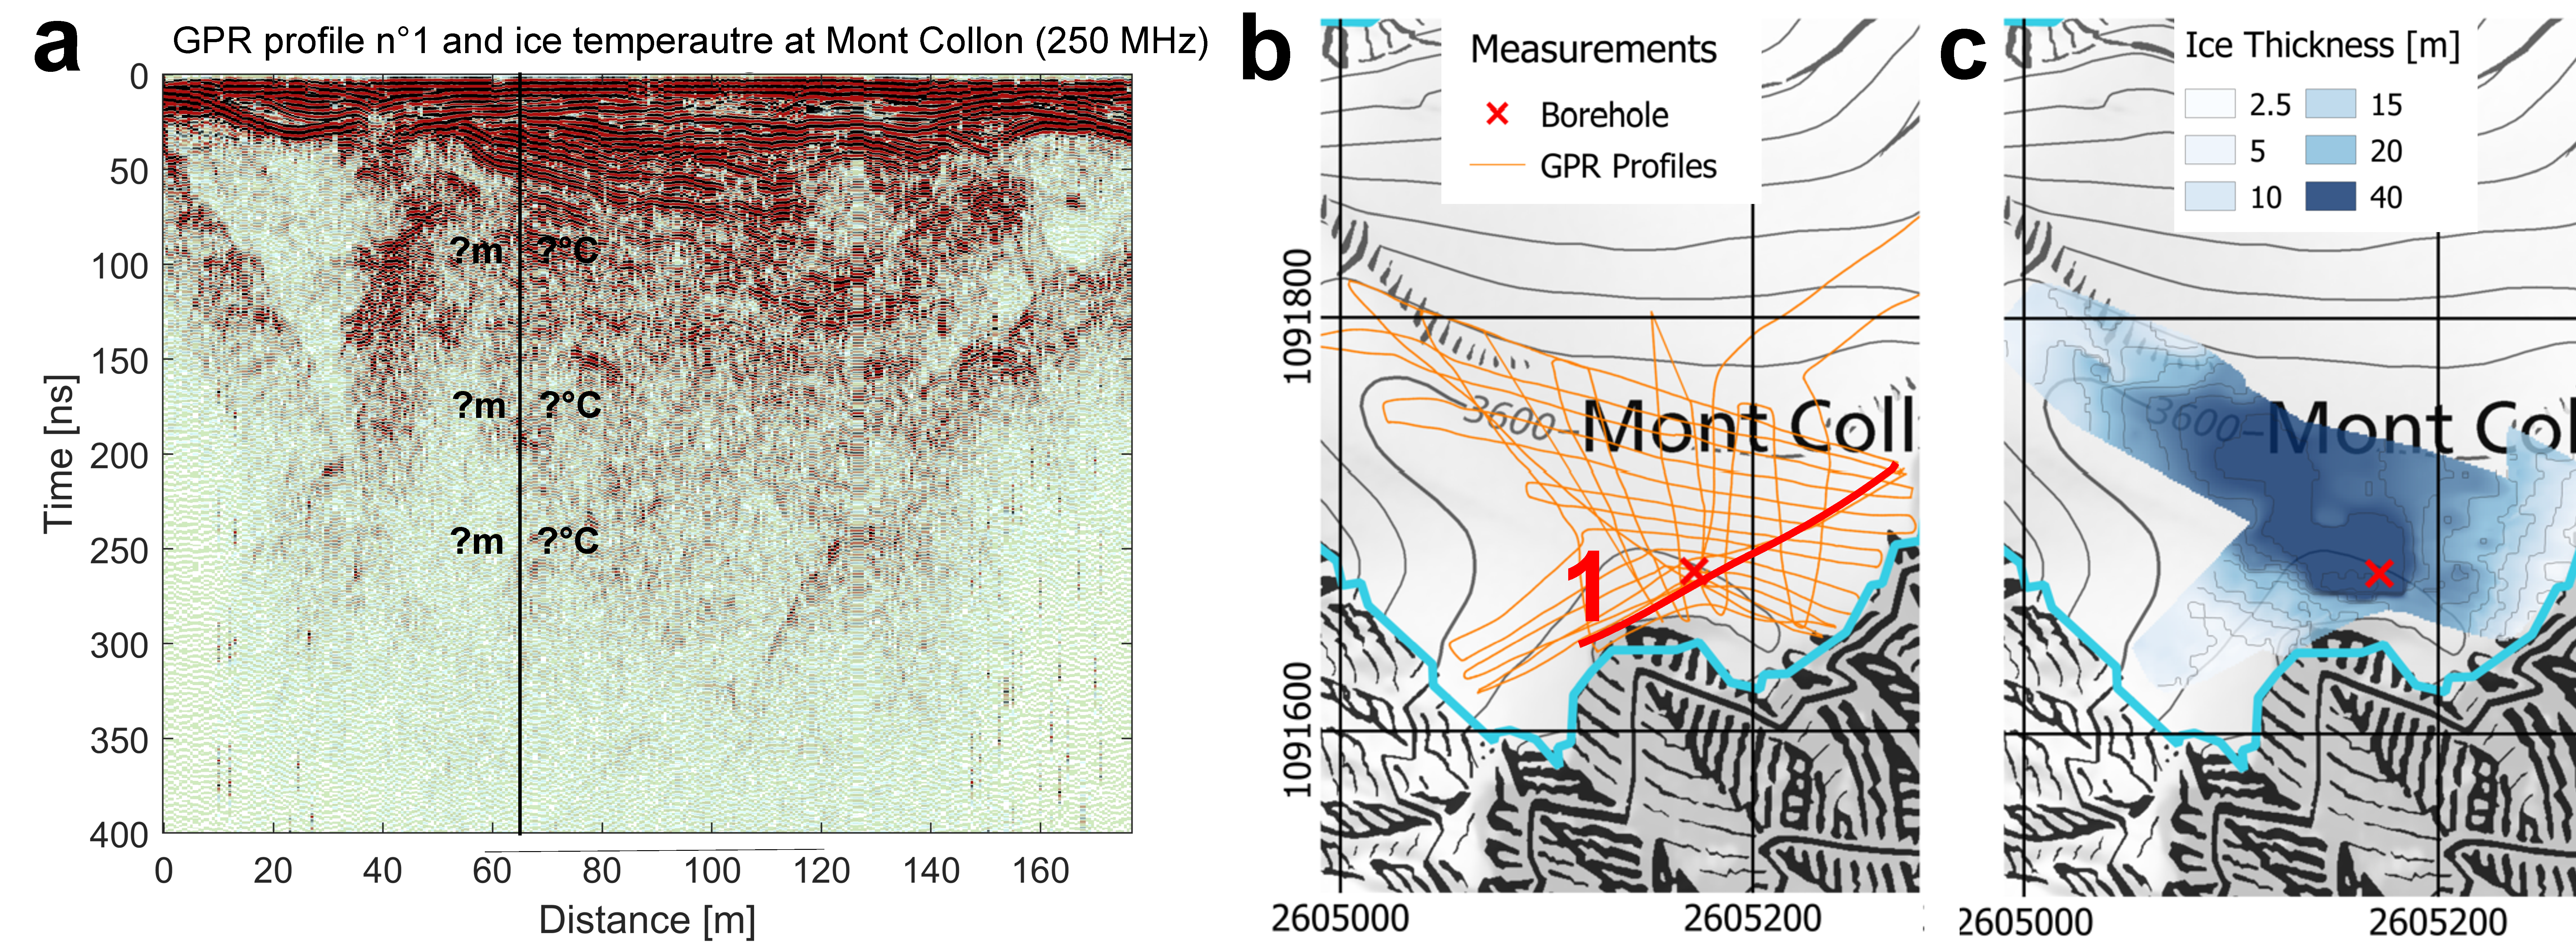
\includegraphics[width=0.9\textwidth]{chapters/Discussion/Collon_GPR.pdf}
    \caption{a) Location of Mont Collon in the Swiss Alps (map from the Federal Office of Topography). The Swiss glaciers are indicated in blue (from the Swiss glacier inventory 2016). b) GPR profiles and boreholes position. c) GPR field data (shown unmigrated) and ice temperature at Mont Collon using a central frequency of 250\,MHz. The time is converted in depth by using a constant electromagnetic velocity in ice of 0.168\,m\,ns$^{-1}$, and the radar field strength is normalized as in Chapter~\ref{ch:chapter_gprmax}). d) Distributed ice thickness at Mont Collon, linearly interpolated from bedrock reflection obtained by GPR measurements. The dash line in c) is a manual representation of the bedrock topography as shown in panel d).}
    \label{fig:collon_GPR}
\end{figure}



\subsection{The use of GPR forward modelling to anticipate complexes GPR field measurements}

In Chapter~\ref{ch:chapter_gprmax}, we used forward modelling of the GPR signal to gain insight in the interpretation of GPR data from field measurements. Here, we further explore additional applications where GPR field measurements could benefit from forward modeling. This approach is particularly advantageous for anticipating complex measurements in remote locations where prior knowledge is essential. After the publication of the Chapter~\ref{ch:chapter_gprmax} \citep{Ogier&al2023}, I co-developed with Barthélémy Anhorn \citep[as part of his master thesis at ETHZ, see][]{Anhorn2024}) an user-friendly python-based package (called gprSlip) to simulate the GPR signal in various context (\url{https://github.com/bart-inho/gprSlip.git}). Our aim was to extend the functionalities of the original gprMax package \citep{Warren&al2016} to accommodate a broader range of geometries, and by consequence to address some of the specific needs for glaciologists and geophysicists. Our package is currently used in two ongoing projects \citep{Aichele&al2024,Mittelholz&al2024}. I present these two applications in the next two subsections, as they highlight the value of forward modelling in applied geophysics (in the first example under a glacier, in the second on the moon). 
%In this regard, forward modelling of the GPR signal could also be used in the future to anticipate fieldwork aiming at locating glacial water pockets. 

\subsubsection{Proof of concept for the imaging of basal stick-slip events using GPR forward modelling}
 
Glacial sliding is a major component of glaciers dynamic, and its understanding is crucial for accurate projection of sea level rise caused by ice sheet melting \citep{Ritz&al2015}. It has been shown that glaciers slide through a series of stick-slip events, characterized by periods of gradual stress accumulation followed by sudden releases of stored energy causing rapid movement \citep{Walter&al2011,Podolskiy&al2016,Grab&al2021}. The ruptures at the origin of the stick-slip can occur entirely in the till, debris or ice layer, or at interfaces between the bedrock/till and the ice. The dominant frictional mechanisms can vary, including viscoelastic till deformation \citep{Tulaczyk&al1999}, velocity strengthening on hard beds \citep{Guerin&al2021}, or rate-and-state friction \citep{Zoet&al2020}. However, little is known about the prevalence and relative significance of these mechanisms in natural settings. 

Glacier sliding has shown seismic evidence of stick-slip motion similar to fault locking \citep{Podolskiy&al2016,Graff&Walter2021}, but these studies show that locating and assessing the extent of stick-slip remains challenging due to low seismic amplitudes. Moreover, in situ monitoring methods relying on boreholes equipped with tilt sensors and cameras have limitations due to the extensive fieldwork required and the poor spatial and temporal resolution achieved. A non-invasive in situ imaging method would be ideal for locating and tracking stick-slip events in space and time with minimal disturbance to the medium. Imaging by non invasive methods can be performed by optical \citep[e.g.][]{Rubino&al2020,Steinhardt&al2022} and ultrasonic methods \citep[e.g.][]{Latour&al2011,Aichele&al2023}. Both methods utilize similar principles: rapid imaging via either light or ultrasound waves determinate the relative displacement between two consecutive "snap-shots", and they use speckles as target to track displacement. Speckle are small scatterers (i.e.\ smaller than the wavelength) that are randomly distributed in the medium. 

In 2023, the SPARK project led by Johannes Aichele and untitled "GPR Icequake Tracking: Non-Invasive Imaging of Glacier Stick-Slip" (SNSF grant 221335, ETHZ, Switzerland), aimed to demonstrate that glacier displacement, both at the bed and within the ice during a stick-slip event, can be quantified using GPR analysis. The scattering observed in the GPR signal correspond to spatial variations in dielectric properties, such as changes in water content or sedimentary debris. While the signal of these speckles are often disregarded as noise or smoothed during post-processing, the project aims to utilize these signals to track glacier displacements. By using a phase-and-speckle tracking algorithm similar to the one used in optics and ultrasound as described in \cite{Aichele2019}, the project aims to monitor individual stick-slip events with the high temporal and spatial resolution required to capture the local and short-term nature of these processes.

As a proof of concept for the project, we used the 2D synthetic GPR signal I performed in Chapter~\ref{ch:chapter_gprmax} as input for the phase correlation algorithm. Specifically, the model of water inclusions presented in Chapter~\ref{ch:chapter_gprmax} were considered as speckles (i.e.\ the target to track) for synthetic imaging of a stick-slip event (see Fig.~\ref{fig:GPR_geometrie_dpl}a). We created a synthetic stick slip by shifting all water inclusions along the vertical, with a Gaussian-gradient like in the displacement amplitude (largest displacements are obtained at the bed)(Fig.~\ref{fig:GPR_geometrie_dpl}b). A vertical displacement means that the vertical phase of the signal aligns with the propagating phase, since the radar wave propagate vertically. The resulting displacement field served as synthetic observations to test the phase-change tracking algorithm in \cite{Aichele2019}. The frequency (25\,MHz) and the time-domain parameters for gprMax simulations and the GPR processing steps are similar as in Chapter~\ref{ch:chapter_gprmax} (see Table~\ref{tab_domain}). The signal phase is ultimately extracted using a Hilbert transform after the Kirchhoff migration.


\begin{figure}[H]
    \centering
    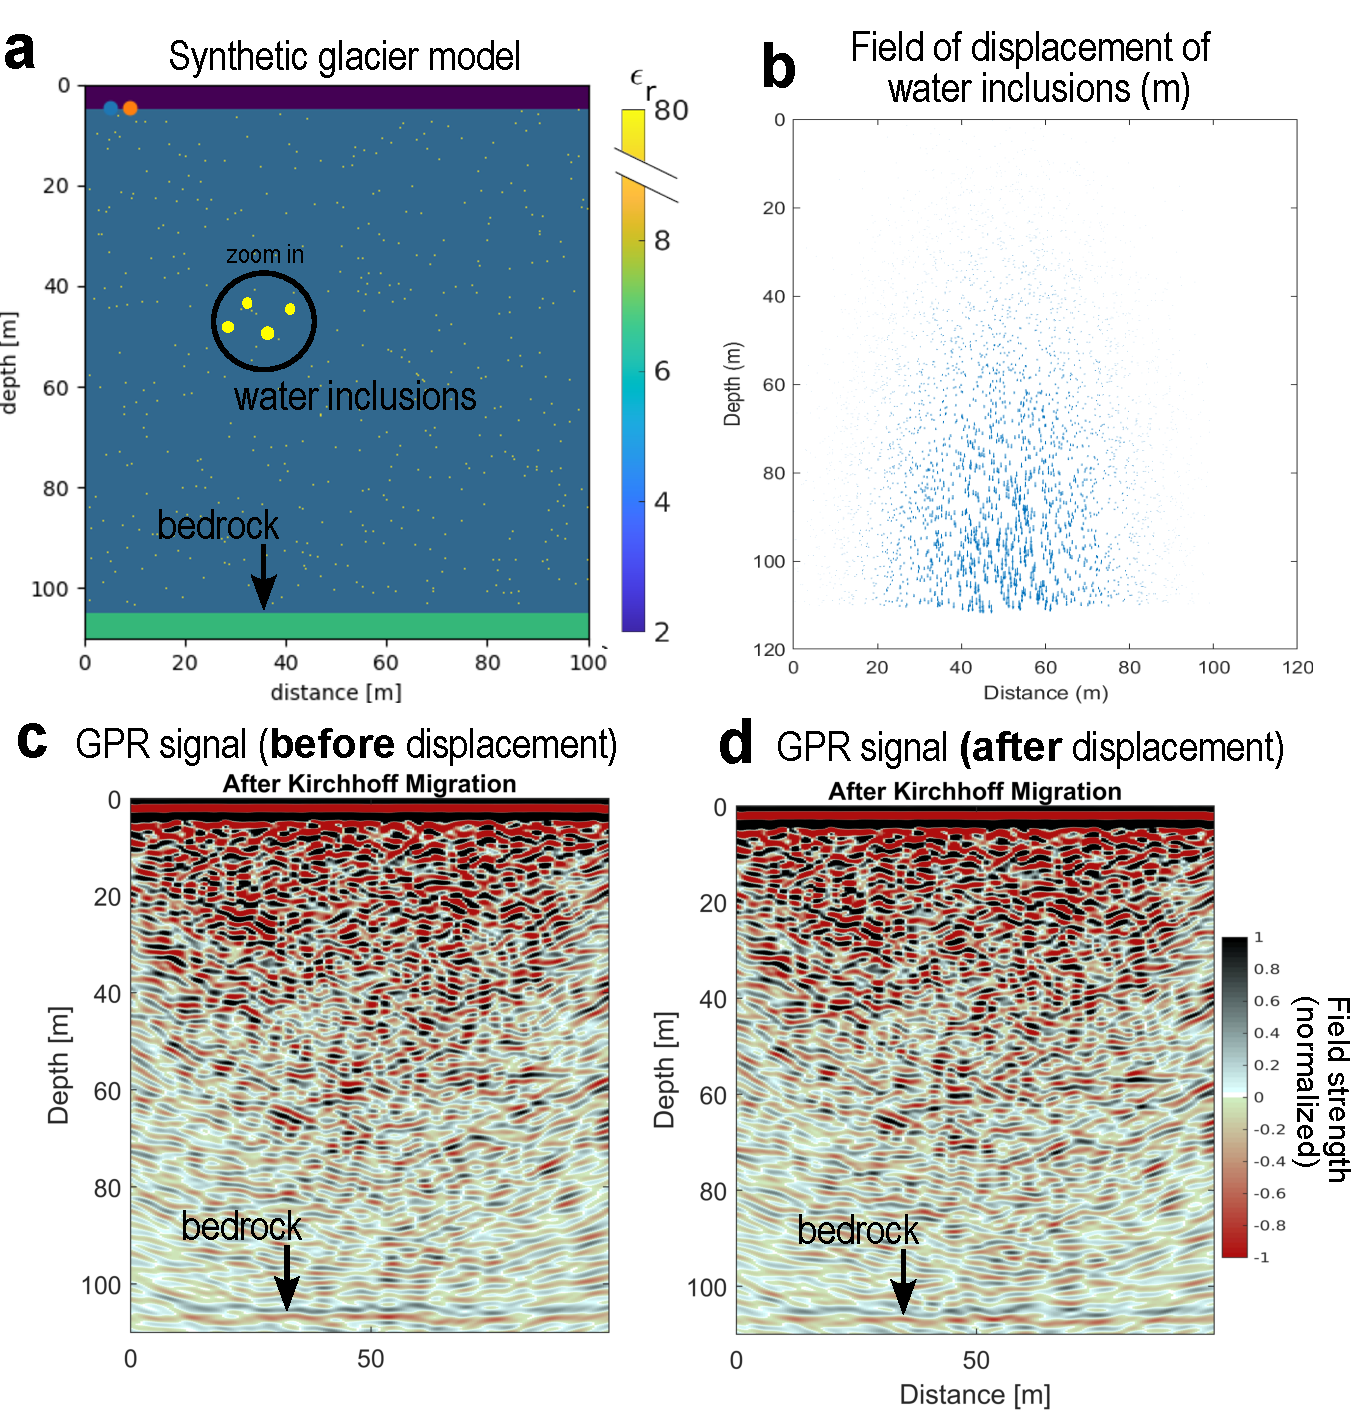
\includegraphics[width=0.7\textwidth]{chapters/Discussion/model_gpr_dpl.pdf}
    \caption{a) Example of a 2D glacier geometry model and relative permittivity ($\epsilon_r$) to simulate a stick-slip event. The initial position of the GPR antennas is shown by the blue (receiver) and red (transmitter) dots. In this model all water inclusions (n\,=\,5000, less is shown here) have a radius of 0.05m, which corresponds to a liquid water content of 0.35\,\%. (b) Field of vertical displacement (arrows) applied to the water inclusions (0.6\,m max). c) Results of the gprMax simulations before displacement and d) after displacement. Results (c) and (d) are presented after Kirchhoff migration and for a central frequency of 25\,MHz.}
    \label{fig:GPR_geometrie_dpl}
\end{figure}


Preliminary results of the forward modelling study were shown at the European Geosciences Union conference in April 2024 \citep{Aichele&al2024}. These qualitative results showed that displacements of 0.6m (i.e.\ $\approx$9\,\% of the radar wavelength in ice at 25\,MHz) at 110\,m depth could be resolved with a accuracy in the order of 0.1/0.2\,m (see Fig.~\ref{fig:GPR_phase}). In the presented example, the amount of water inclusions correspond to a liquid water content 0.35\,\%, which falls in the typical range of liquid water content in mountain glacier (see Section~\ref{sec:LWC_GPR} in \citep{Ogier&al2023}).


\begin{figure}[H]
    \centering
    \includegraphics[width=0.8\textwidth]{chapters/Discussion/GPR_dpl_phase.pdf}
    \caption{Results from \cite{Aichele&al2024} (with permission) showing a) the reconstructed water inclusions vertical displacement (dpl) from the phase correlation algorithm (left), showing vertical profiles at x\,=\,100\,m and x\,=\,130\,m (right), and b) synthetic vertical displacement of water inclusions of the input model (left), showing vertical profiles at x\,=\,100\,m and x\,=\,130\,m (right). The input model for the displacement of water inclusion can also be visualized in Figure~\ref{fig:GPR_geometrie_dpl}b}
    \label{fig:GPR_phase}
\end{figure}

Results from \cite{Aichele&al2024} (with permission) showing (a) the reconstructed vertical displacement (dpl) of water inclusions from the phase correlation algorithm, depicting vertical profiles at x=100 and x=130 (right panels corresponding to Fig.~\ref{fig:GPR_geometrie_dpl}c and d), compared to (b) the synthetic vertical displacement of water inclusions in the input model."

Following these results, field measurements at Grenzgletscher (Switzerland) were conducted in March 2024 in the frame of the project (I was not involved in the fieldwork). As a radar system, an autonomous phase-sensitive radio echo sounder (APRES) is used to directly retrieve the phase of the signal, discarding the need for the Hilbert transform step required when using GPR. Additionally, APRES provides a better spatial resolution, unlike GPR which measures specular reflections and cannot resolve target smaller than half of the wavelength in the medium \citep{Davis&Annan1989}. The APRES unit was coupled with 16 antennas deployed in line. The choice of the APRES frequency directly influences the maximum displacement detectable, as phase changes up to 1\,\% of the dominant radar wavelength can be theoretically tracked with the APRES \citep{Nicholls&al2015}. The APRES used modulated frequencies ranging from 250\,MHz to 400\,MHz, which should provide a spatial resolution in ice of the order of mm. This spatial resolution should be in theory sufficient to track stick-slip events at the glacier base. Indeed, the displacement caused by individual stick-slip events was estimated to range from micrometers (in ice) to millimeters (at the ice-till interface), which can sum up to centimeters per day \citep{Graff&al2021}. Data was recorded for two weeks. Several challenges in processing the field data are expected to arise. For instance, the displacement patterns may not align purely vertically, as represented in our synthetic models. Additionally, there are other factors that can influence the radar signal for relatively short time scale and which are challenging to constrain, such as fluctuations in liquid water content. Currently, the signal is being analyzed by Aichele, with the goal of reproducing similar results as shown in Figure~\ref{fig:GPR_phase} for one vertical profile at the APRES location. Meanwhile, we plan to conduct additional numerical simulations that incorporate horizontal displacement, rather than purely vertical movements. These simulations will be discussed in a publication (in preparation).

\subsubsection{The use of GPR forward modelling prior to field measurements on the moon}

We present here another project (LunarLeaper), where our forward numerical modelling of the GPR signal presented in Chapter~\ref{ch:chapter_gprmax} contributes to its advancement. LunarLeaper is a conceptual robotic explorer designed for lunar missions, in response to the ESA 2023 Small Missions call. The robot concept was presented at the European Union Geosciences in 2024 \citep{Mittelholz&al2024}. LunarLeaper will use a GPR and a gravimeter to conduct detailed surveys of the subsurface. The mission aims to investigate and confirm the presence of former lava tubes (now sub-surface voids) that could potentially serve as sites for future human exploration on the Marius Hills pit \citep{Wagner&al2014,Sauro&al2020}. GPR will provide high-resolution images of the subsurface structure to map the geometry of potential voids and assess the pit's stability. 
%
To anticipate the potential field results of the mission, I conducted forward GPR modeling at 500 MHz using our package gprSlip in a typical lunar surface scenario: a basal layer beneath a five-meter-thick regolith layer at the surface. Regolith, characterized by its resistive properties \citep{Ding&al2022}, is expected to strongly attenuate the amplitude of GPR signals. We performed two test: one GPR model without regolith and one with regolith. The model without regolith produced perfectly clear reflection from the lunar pit (Fig.~\ref{fig:lunar_pit}a), while the model with regolith showed significant attenuation (Fig.~\ref{fig:lunar_pit}b), although the lunar pit located 20 meters beneath the surface was still detectable. These findings suggest that, despite the attenuating effects of the regolith, voids should theoretically be detectable but challenging. Note that the high frequency used in the simulations would be likely responsible for strong attenuation of the signal in the field. In conclusion, the GPR forward modelling conducted in this thesis helped to discuss the relevance of the GPR in detecting lunar pits prior to the actual field measurements. We recommend more theoretical work to obtain a better a priori knowledge from the LunarLeaper mission, in particular to assess the influence of the GPR frequency to the signal.  


\begin{figure}[H]
    \centering
    \includegraphics[width=0.7\textwidth]{chapters/Discussion/lunar_pit.pdf}
    \caption{Synthetic lunar pit geometries and its gprMax results corresponding to lunar soil a) without regolith and b) with regolith.}
    \label{fig:lunar_pit}
\end{figure}


%\subsection{Water pockets detection using GPR}


% \begin{itemize}
%     \item Suitable or not? For which strategies? 
%     \item Alternatives to explain limitations in data interpretation: rock inclusions (see Ilaria's work)
%     \item Few words on the potential of airborn-GPR analysis by Ilaria
% \end{itemize}

% \section{The future of GLOFs research}

% \todo{is it even necessary? or the conclusion is enough?}

% Form this chapter discussion: we put light on future directions: more field measurements and modelling (the use of recently acquired data set to validate modelling studies), more monitoring of WP, in particular by combining geophysics

%Discussion on GLOFs:

%\cite{Carrivick&Tweed2016}: This problem leads us to make key recommendations that there needs to be accurate, full and standardised monitoring and recording of glacier floods, in particular to preferably discriminate flood volume and peak discharge at source rather than at some distance down valley. Otherwise the physical mechanisms responsible for generation of the flood are masked by the effects of channel topography on flood evolution with distance down valley.

%\cite{Emmer&al2022}: research on GLOFs include more and more co-authors (= increase in collaboration), and show 30\% of international collaboration (our WPOFs paper fits in).


% Discussion on the future occurence of GLOFs and WPOFs
% link with climate change and glacier retreat (more proglacial lakes, less ice to store WP?)
% example in role of climate and climate change (Zheng et al., 2021b)(cited in Emmer 2022)


% thermal regime is important for water pocket. Thermal regime can be characterized by GPR. DIscuss Alphubel and mont collon findings in this regard. 

%Interesting: Veh et al (2022) reported 312 (219 GLOFs) for the Swiss Alps (from 1560 to 2019), we report 92 WPOF. Hence, 30% of the glacier flood (n=312) are WPOF, so Haberli's statement that 30/40& of glacier flood are from water pocket stands. -> phenoman frequent and needs observations to be better understood


% to quantify WP growing VS closure, the former being slower than the latter.  From Manu: "the kinetics of clossure is much higher (proportionnal to the cube of the ice pressure) than the kinetics of openning (proportionnal to the cube of the difference of ice and water pressures)"

% return period of WPOFs according to their magnitude

% Bias is a big thing in GLOFs reporting. What about WPOFs?

% we found that WPOF occur every 6 years in average since 1900, but we miss most of the events. A case study could be quantify better the real occurence of water pocket filling and bursting

% we need a monitoring of (at least) one of the WP mechanism identified in Ogier et al 2024!

% what is needed to understand GLOFs from surface lakes? highlight again the Gag's study outcomes on Bossons 

% discussion topic: 
%1) we got some better parametrization -> what's next to really well model surface glacier lake drainage? -> validation/calibration on case study
%2) we know water inclusions matter: what should we do on the field?
%3) we characterized WP, what's next? -> more monitoring, thermal regime, etc...

%Strategies for detecting alpine water pockets

% \begin{itemize}
%     \item Several projects ongoing to detect water pocket:
%     \item SNMR by Laura G.
%     \item Passive seismic
%     \item Glacier thermal modelisation by Juliette Bonnet (IGE)
%     \item Teledection technique was not used in this thesis, but has interesting potential for WP detection
%     \item positive anomaly of MB time series as a favorable factor (see Tête Rousse in 1892)?
%     \item combine with output on the GPR of the next section?
% \end{itemize}

%early warning system:
%comMF: maybe one could also say that real-time discharge measurements in proglacial streams could at least for some WPOF mechanisms (temporary blockage of subglacial channels) be used for early warning for downstream areas (i.e. if unexpected drop or cut-off in discharge occurs), as we show that this mechanism occurs quite frequently (resp. is the most frequent WPOF mechanism that we detected)...

%Daniel: Don't ask me why I think of it only now, but here I was suddenly wondering: in which of the 4 mechanisms that we propose would this fit? I guess it is closest to "water filled crevasse", although it is not a crevasse at all. Does it mean that we need a 5th mechanism?  [Ok, later in the article I saw that, indeed, this was counted towards "water-filled crevasse"). And as I think of it: did Mauro H. (or someone else) correlate the number of WPOFs to MB? I suddenly start to like the idea that there might be "relictic lakes" buried within glaciers ;-) Possibly Ilaria could look up old aerial images and see whether there are anomalous GPR signals at locations where supraglacial lakes existed in periods of positive MB? It's av bit of a hair-pulled hypothesis, I admit (lakes would get advected by ice flow, and when doing so, they might drain anyway), but somehow, we still don't really have a clue how WPs form.
% -> yes this crossed my mind 3 years ago. 


% outlook: to look at slope geometry dowstream glacier and the presence of lake as correlation with the occurence of WPOF. WOuld that tell something on the observation biases? in particular would that explain the spatial pattern of reported WPOFs?




%\subsection{Other}

%matthias: The shift from the observation by Haeberli that most events come from steep glaciers in comparison to our analyis might be due to a difference in the dominant types that has been induced by climate change - roof-collapses are increasingly observed now. For example, steep glaciers are unlikely to qualify for the roof-collapse type, whereas valley glaciers are unlikely to relate to the Tete-Rousse case (polythermal ice). The shift from the observation by Haeberli that most events come from steep glaciers in comparison to yours might be due to a difference in the dominant types that has been induced by climate change - roof-collapses are increasingly observed now.
% -> I think this a too weak statement. In fact, temporary blockage are inventoried all along the century, without a particular trend


% Some consideration as comments on the role of overdeeping in WPOFs:
%The drainage system of Findelen is mostly inefficient and distributed \citep{Swift&al2021,Iken&Bindschadler1986}. This might play a role in the occurrence and the frequency of these little outburst events. And sometimes, like in 2017, the temporary blockage is larger/longer than usual, and can accumulate larger volume (e.g. ~17 000 m3) and the ice dam break lead to an outburst, a so-called water pocket outburst flood.
%\cite{Hooke&Pohjola1994} indicate that Shreve's law breaks down near overdeepening and that water might route from subglacial conduit to englacial conduit in overdeepening as a response of the adverse slope. In adverse bed slope, the water freeze when most of the energy is stored as potential energy, and the subglacial pathway blocks. Because in steep adverse slopes, the energy form viscous dissipation is not enough to warm the water, which is needed since the melting point rises in response of the falling pressure. In addition, they suggest lenticular conduits with, importantly, local constriction along the way to support their observations. These local constriction could be potential location for water pocket (that is what Swift 2021 say between the lines of their introduction: another example of water pocket as "linked subglacial cavities of a distributed system"). 

%Note really relevant for the hydraulic barrier section:
%Note that the same topographic feature (i.e.\ a glacier surface depression, see Fig.~\ref{fig:plainemorteWP}) that is prone to subglacial water pockets formation is also prone to form moulins. For moulins, the subglacial hydraulic barrier is hydraulically connected to the glacier surface. Therefore, the water reservoir is not entirely subglacial but mostly supraglacial and at atmospheric pressure. If the hydraulic barrier is located along the subglacial drainage pathways that generally form during the melt season \citep{Fountain&Walder1998}, the water will be drained through the subglacial drainage network before the water pocket can form. In general, subglacial channels that form early in the melt season remain connected to the subglacial drainage system throughout the melt season. For subglacial channels remaining open during the whole melt season, the development of a water pocket at locations of hydraulic barriers is therefore unlikely. 

%We relate the fact that temporary blockage of subglacial channel is the WPOFs mechanism the most represented in our inventory with the fact that most of the WPOFs also occurred after a few days-long positive temperature anomaly (see Section~\ref{sec:envelop}). One can speculate that in the observed period of maximal positive temperature anomalies (i.e.\ , during the five days prior to the WPOF), the subglacial network experiences very high fluctuations in discharge. We suggest that these fluctuations can exert considerable mechanical work on the roof of conduits, potentially weakening it. When the water levels drop in the late afternoon or night, the conditions would be given for parts of the roof to collapse into the partially empty channels. This can block the channel temporarily until the next meltwater comes, builds up water pressure, and eventually causes the blocking to let go at once.


% Interesting comment from Manu: "what we have learned from Tête Rousse is that the opening of a water pocket is far much slower than a closure process when water has been drained. Therefore I understand that a filling by precipitation in hours or days  can play a role under the condition of a pre-existing cavity."


%One important thing relates to the mechanisms to store water: for (1), (2) and (3), existing voids are necessary that can be quickly filled without the need for further growth of the water reservoir when it is full of water. For (4), initial voids are not necessary, just some en-/subglacial water connection upstream the thermal barrier, and then the reservoir grows by ice creep due to high water pressure.







% EXTRA not published:

% \subsection{ A metric for the prevalence of low hydraulic slopes on glaciers}


% Here we present how we calculate the relative proportion of areas of low hydraulic potential gradient for all Swiss glaciers used in Section~\ref{sec:prediction} to complete \cite{Hupfer2023}.

% The map-plane gradient of the hydraulic potential $\nabla\,\psi$ is the vector
% %
% \begin{equation}
%      \nabla\,\psi = \left(\frac{\partial\,\psi}{\partial x}, \,\,\frac{\partial\,\psi}{\partial y}\right),
%      \label{eq:grad_phi_formula}
% \end{equation}
% %
% where $x$ and $y$ are the horizontal coordinates. 
% The L2-norm of the gradient of the hydraulic potential $\vert \nabla\,\psi \vert $ is equal to
% %
% \begin{equation}
%     \vert \nabla\,\psi \vert  = \sqrt{\left(\frac{\partial  \psi}{\partial x}\right)^2 + \left(\frac{\partial \psi}{\partial y}\right)^2}.
%      \label{eq:norm_grad_phi}
% \end{equation}
% The norm of the Shreve potential can then be calculated by substituting Equation~(\ref{eq:phi}) into the previous two equations.

% %
% %Given the equation above, surface slope is approximately ten times more important than bed slope to drive water flow at the glacier bed. This means that water can flow against reverse slope of overdeepening, as long as the bed slope is less than $\approx$10 times steeper than the surface slope. 

% We calculate the area for individual glaciers where $\vert \nabla\,\psi \vert $ is lower than 4\,\%. This threshold value is arbitrarily chosen after visualisation on a geospatial information system to isolate areas of low hydraulic gradient where water is more likely to accumulate. For each glaciers, we normalise this area by the glacier area. The higher this variable, the higher the relative proportion of area having a low hydraulic slope. 
% %Hypotheses behind: the biggest proportion of inefficient drainage area within a glacier, the most likely water accumulates, and thus water pocket to form. 

% The distributed map of the gradient-norm of the hydraulic potential for all Swiss glacier can be downloaded at \todo{link to ETHZ collection}.


%Discussion on Bosson and the DH length. In \citet{Emmer&al2022}: suggest as further research to back-calculating relevant events in order to refine model parameters and define plausible sets of parameters for predictive modelling of potential future events. That is what Gag does here with my dataset.